\chapter{Method}
The design and prototype iterations of the haptic metronome are discussed extensively throughout Appendix \ref{designReq} along with a parts list and schematic of the hardware builds.\footnote{All of the code is open source and readily available at \url{https://github.com/afaintillusion/he-sm}}

This chapter outlines each test case and describes the motivation behind the test plan. Furthermore, it briefly delves into the test suite design and calculates a round-trip latency of the system in order to find a close approximation of relative accuracy. The hope is to establish a level of confidence in the precise time dependent information.

The overall test principle was derived from traditional sensorimotor synchronization tasks in which a user is asked to tap to a corresponding stimulus. The asynchrony was tracked and plotted along with the \textit{PCR} and any missed taps. Since the haptic domain is of primary focus, the auditory modality functions primarily as a benchmark or baseline foundation. The work presented in \ref{visualMet} covers the idea of the interstitial beat occupying the visual domain and as such will not be re-evaluated here.

Each test case is defined and presented in \ref{testPlan}. The overall software development process is detailed in \ref{development}. The test suite is discussed in \ref{tap_arduino} and latency calculated in \ref{latencyCalc}.

\section{Test Plan} \label{testPlan}
Testing was divided into two major sections, \textbf{Steady} and \textbf{Dynamic}, implying either an \textit{isochronous} or a \textit{non-isochronous} pulse respectively. While structurally identical, the dynamic tests however focussed on rubato within a range starting at the predefined BPM and rising or falling within a specified window (maximum span of +/- 15 bpm). The chosen tempi parallels slow walking to running gaits spanning a range of 45-180 beats per minute.

Each section has three subsections centered around either an audible metronome tone (\textbf{A1, A3}), musical note (\textbf{A2, A4}), and lastly the haptic modality (\textbf{H1, H2}). Subsections were further broken down into \textbf{a} and \textbf{b}, denoting either \textit{discrete} or \textit{interstitial} (\textit{continuous}) mode of operation. A breakdown of the test plan is shown in Figure \ref{fig:TestPlan}. The data analysis in Chapter \ref{DataAnalysis} will frequently reference this table as a legend.

As discussed in Appendix \ref{designReq}, the haptic was designed with two operating modes in mind, discrete and continuous. These modes were programmatically controlled to match the desired test cases, extensively explained in section \ref{development}.
\begin{table}[t]
    \centering
    \resizebox{\textwidth}{!}{%
        \begin{tabular}{cclllcclll}
        \hline
        \multicolumn{10}{c}{\cellcolor[HTML]{000000}{\color[HTML]{FFFFFF} Steady}} \\ \hline
        \multicolumn{3}{c}{Discrete} & BPM & \multicolumn{1}{l|}{Runtime (sec)} & \multicolumn{3}{c}{Interstitial} & BPM & Runtime (sec) \\ \hline
        &  & i. & 45 & \multicolumn{1}{l|}{20} &  &  & i. & 45 & 30 \\
        &  & ii. & 90 & \multicolumn{1}{l|}{20} &  &  & ii. & 90 & 16 \\
        &  & iii. & 135 & \multicolumn{1}{l|}{20} &  &  & iii. & 135 & 11 \\
        \multirow{-4}{*}{A1a} & \multirow{-4}{*}{click} & iv. & 180 & \multicolumn{1}{l|}{20} & \multirow{-4}{*}{A1b} & \multirow{-4}{*}{legato chime (swing click)} & iv. & 180 & 8 \\ \hline
        &  & i. & 45 & \multicolumn{1}{l|}{32} &  &  & i. & 45 & 32 \\
        &  & ii. & 90 & \multicolumn{1}{l|}{16} &  &  & ii. & 90 & 16 \\
        &  & iii. & 135 & \multicolumn{1}{l|}{11} &  &  & iii. & 135 & 11 \\
        \multirow{-4}{*}{A2a} & \multirow{-4}{*}{staccato music (melody)} & iv. & 180 & \multicolumn{1}{l|}{8} & \multirow{-4}{*}{A2b} & \multirow{-4}{*}{legato music (melody)} & iv. & 180 & 8 \\ \hline
        &  & i. & 45 & \multicolumn{1}{l|}{15} &  &  & i. & 45 & 15 \\
        &  & ii. & 90 & \multicolumn{1}{l|}{15} &  &  & ii. & 90 & 15 \\
        &  & iii. & 135 & \multicolumn{1}{l|}{15} &  &  & iii. & 135 & 15 \\
        \multirow{-4}{*}{H1a} & \multirow{-4}{*}{poke / all on (instantaneous)} & iv. & 180 & \multicolumn{1}{l|}{15} & \multirow{-4}{*}{H1b} & \multirow{-4}{*}{oscillate down and back up} & iv. & 180 & 15 \\ \hline
        \multicolumn{10}{c}{\cellcolor[HTML]{000000}{\color[HTML]{FFFFFF} Dynamic}} \\ \hline
        \multicolumn{3}{c}{Discrete} & BPM & \multicolumn{1}{l|}{Runtime (sec)} & \multicolumn{3}{c}{Interstitial} & BPM & Runtime (sec) \\ \hline
        &  & i. & 45 +/- 15 & \multicolumn{1}{l|}{20} &  &  & i. & 45 +/- 15 & 20 \\
        &  & ii. & 90 +/- 15 & \multicolumn{1}{l|}{10} &  &  & ii. & 90 +/- 15 & 10 \\
        &  & iii. & 135 +/- 15 & \multicolumn{1}{l|}{10} &  &  & iii. & 135 +/- 15 & 10 \\
        \multirow{-4}{*}{A3a} & \multirow{-4}{*}{click} & iv. & 180 +/- 15 & \multicolumn{1}{l|}{10} & \multirow{-4}{*}{A3b} & \multirow{-4}{*}{legato chime (swing click)} & iv. & 180 +/- 15 & 10 \\ \hline
        &  & i. & 45 +/- 15 & \multicolumn{1}{l|}{30} &  &  & i. & 45 +/- 15 & 30 \\
        &  & ii. & 90 +/- 15 & \multicolumn{1}{l|}{15} &  &  & ii. & 90 +/- 15 & 15 \\
        &  & iii. & 135 +/- 15 & \multicolumn{1}{l|}{10} &  &  & iii. & 135 +/- 15 & 10 \\
        \multirow{-4}{*}{A4a} & \multirow{-4}{*}{staccato music (melody)} & iv. & 180 +/- 15 & \multicolumn{1}{l|}{10} & \multirow{-4}{*}{A4b} & \multirow{-4}{*}{legato music (melody)} & iv. & 180 +/- 15 & 10 \\ \hline
        &  & i. & 45 +/- 10 & \multicolumn{1}{l|}{15} &  &  & i. & 45 +/- 10 & 15 \\
        &  & ii. & 90 +/- 5 & \multicolumn{1}{l|}{15} &  &  & ii. & 90 +/- 5 & 15 \\
        &  & iii. & 135 +/- 3 & \multicolumn{1}{l|}{15} &  &  & iii. & 135 +/- 3 & 15 \\
        \multirow{-4}{*}{H2a} & \multirow{-4}{*}{poke / all on (instantaneous)} & iv. & 180 +/- 1 & \multicolumn{1}{l|}{15} & \multirow{-4}{*}{H2b} & \multirow{-4}{*}{oscillate down and back up} & iv. & 180 +/- 1 & 15 \\ \hline
        \end{tabular}%
    }
    \caption{Test Plan}
    \label{fig:TestPlan}
\end{table}

\subsection{Subjects}
Out of 18 subjects tested, 16 were parsed to equivalently divide the groups into 8 professionals and 8 amateurs/non-musicians. Usernames were anonymized into User ID's using a cumulative char to int conversion method. A breakdown of the grouping per instrumentation is shown in Table \ref{fig:SubjectTable}.
\begin{table}[t]
    \centering
    \resizebox{.5\textwidth}{!}{%
    \begin{tabular}{|l|l|l|}
    \hline
    \rowcolor[HTML]{000000} 
    {\color[HTML]{FFFFFF} Group} & {\color[HTML]{FFFFFF} Instrument} & {\color[HTML]{FFFFFF} User ID} \\ \hline
     & Bass & 729 \\ \cline{2-3} 
     & DJ & 390 \\ \cline{2-3} 
     & Piano & 399 \\ \cline{2-3} 
    \multirow{-4}{*}{Amateur} & Voice & 379 \\ \hline
     &  & 486 \\ \cline{3-3} 
     &  & 514 \\ \cline{3-3} 
     & \multirow{-3}{*}{None} & 932 \\ \cline{2-3} 
    \multirow{-4}{*}{Neither} & Piano & 394 \\ \hline
     &  & 410 \\ \cline{3-3} 
     &  & 591 \\ \cline{3-3} 
     & \multirow{-3}{*}{Flute} & 824 \\ \cline{2-3} 
     &  & 367 \\ \cline{3-3} 
     &  & 506 \\ \cline{3-3} 
     &  & 521 \\ \cline{3-3} 
     & \multirow{-4}{*}{Percussion} & 552 \\ \cline{2-3} 
    \multirow{-8}{*}{Professional} & Piano & 510 \\ \hline
    \end{tabular}%
    }
    \caption{Subject Grouping}
    \label{fig:SubjectTable}
\end{table}

\subsection{Audio File Generation}
All tracks were rendered using the digital audio workstation (DAW) \textit{Logic Pro X} as \textit{.wav} files at a 44.1kHz sample rate with 16 bit resolution.

\subsubsection{Metronomic click and legato chime}
\textbf{A1a} and \textbf{A3a} required a standard metronomic pulse. This was accomplished using the default Klopfgeist (metronome) plugin from Logic Pro X. No additional tuning was modified and the tonality was left at 0.83 of unity.

\begin{figure}[H]
    \centering
    \caption{Modified click parameters for interstitial tests.}
        \subfloat[Modified metronome]{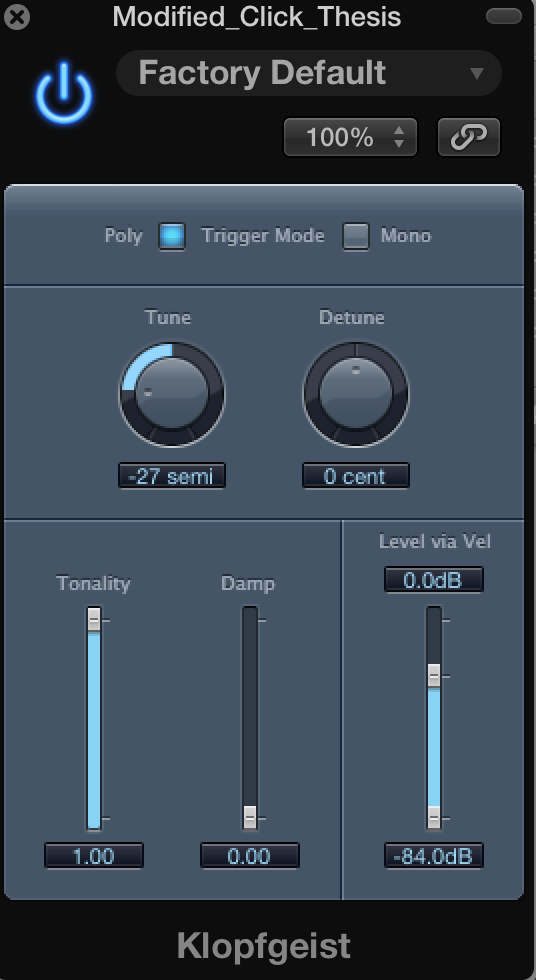
\includegraphics[width=0.25\columnwidth]{Klopfgeist_Modified}}
        \qquad
        \subfloat[Superimposed tremolo]{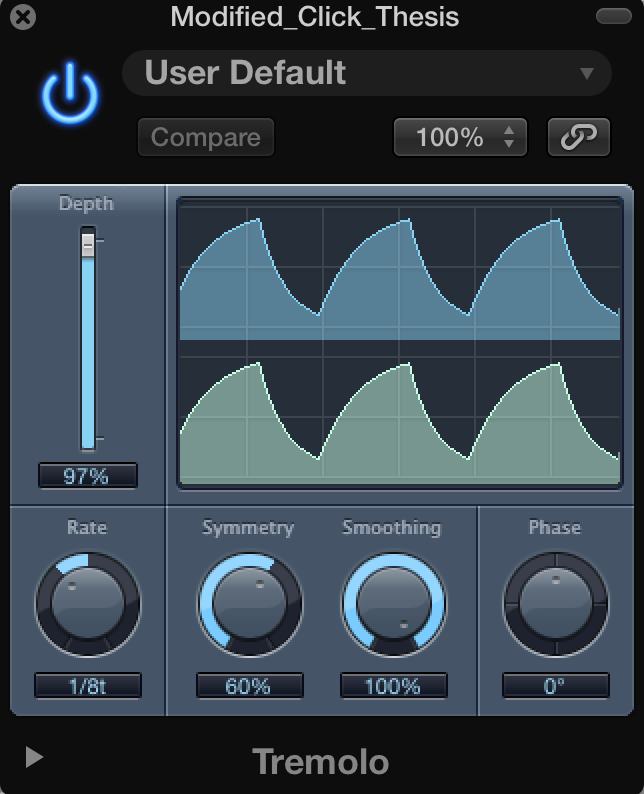
\includegraphics[width=0.4\columnwidth]{Tremolo}}
        \qquad
        \subfloat[Equalized tone]{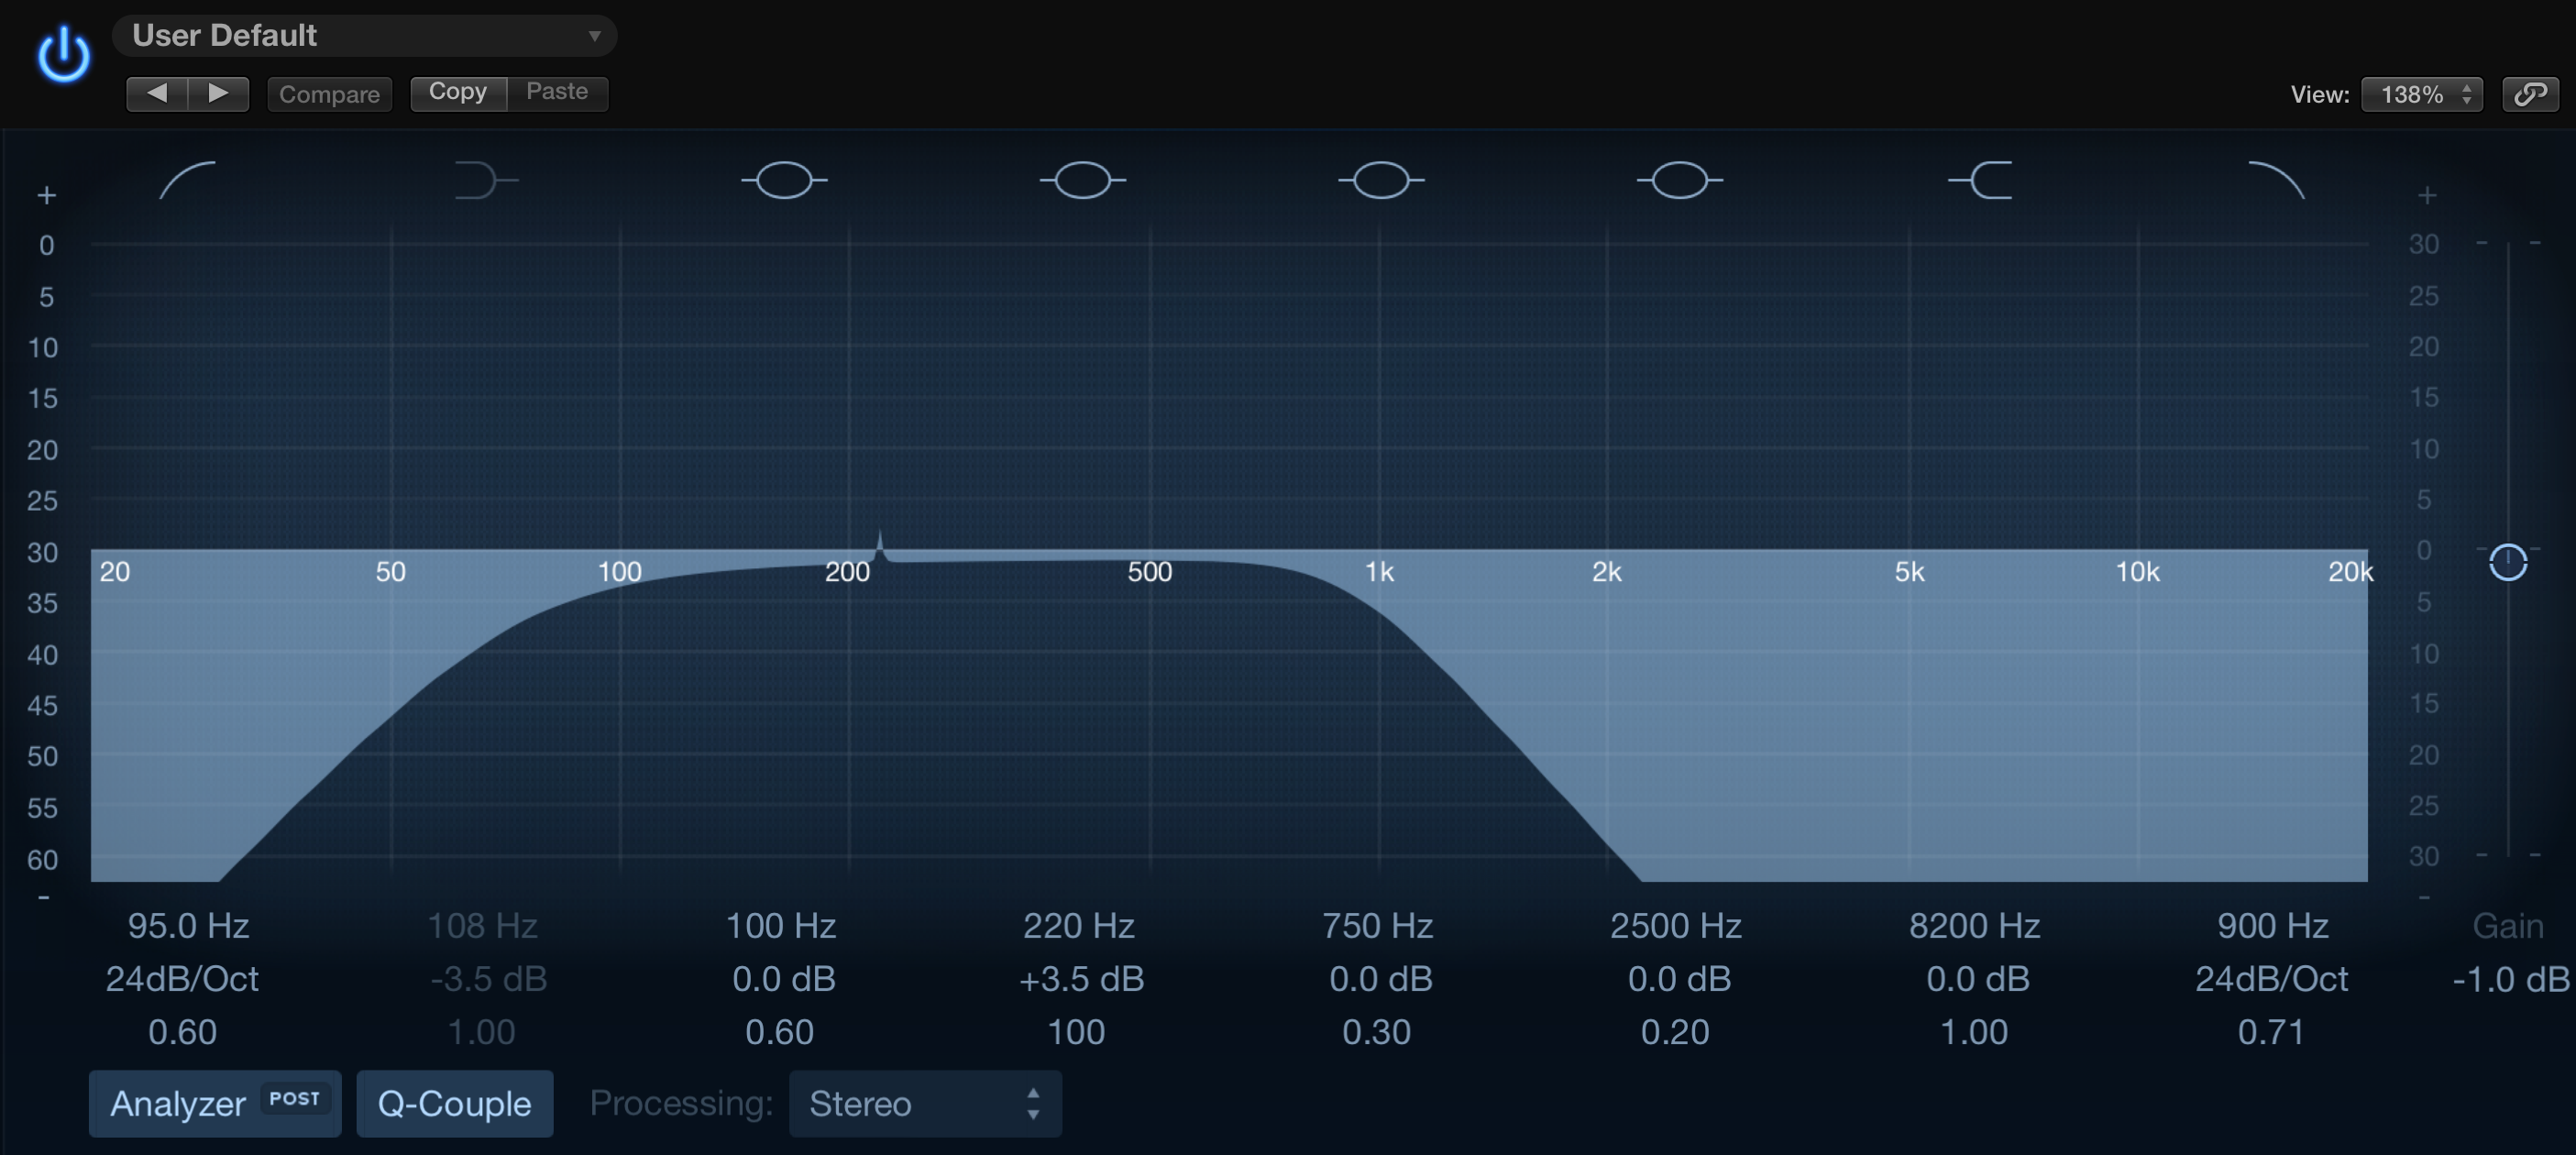
\includegraphics[width=\textwidth,height=0.25\textheight]{Modified_Click_EQ}}
    \label{fig:modClick}
\end{figure}

\textbf{A1b} and \textbf{A3b} however required a swing or legato type of chime in order to convey filling the interstitial space. To capture this effect the Klopfgeist tonality was increased to unity and tuned -27 semitones lower which served to both soften diminish the discrete click, provided an elongated or continuous audible sensation. 

To give the impression of a sound that was ramping up in amplitude and decaying after the peak, a tremolo effect which mimics a sawtooth wave was added to the signal chain as seen in Figure \ref{fig:modClick}. 

Last, a multi-band EQ was placed at the end of the signal chain with a bandpass filter from 95Hz-750Hz removing any unwanted frequency presence with a 3.5dB high-Q peak at 220Hz to emphasize the tonality.

The resultant waveform encapsulated the occupation of the interstitial space. A comparison of this waveform in contrast to it's discrete counterpart is shown in \ref{fig:click_comparison}. Note the envelope of signal (b) follows a natural build up and decay.

\begin{figure}[H]
    \centering
    \caption{Metronomic waveform comparison}
        \subfloat[A3a1: discrete audible click]{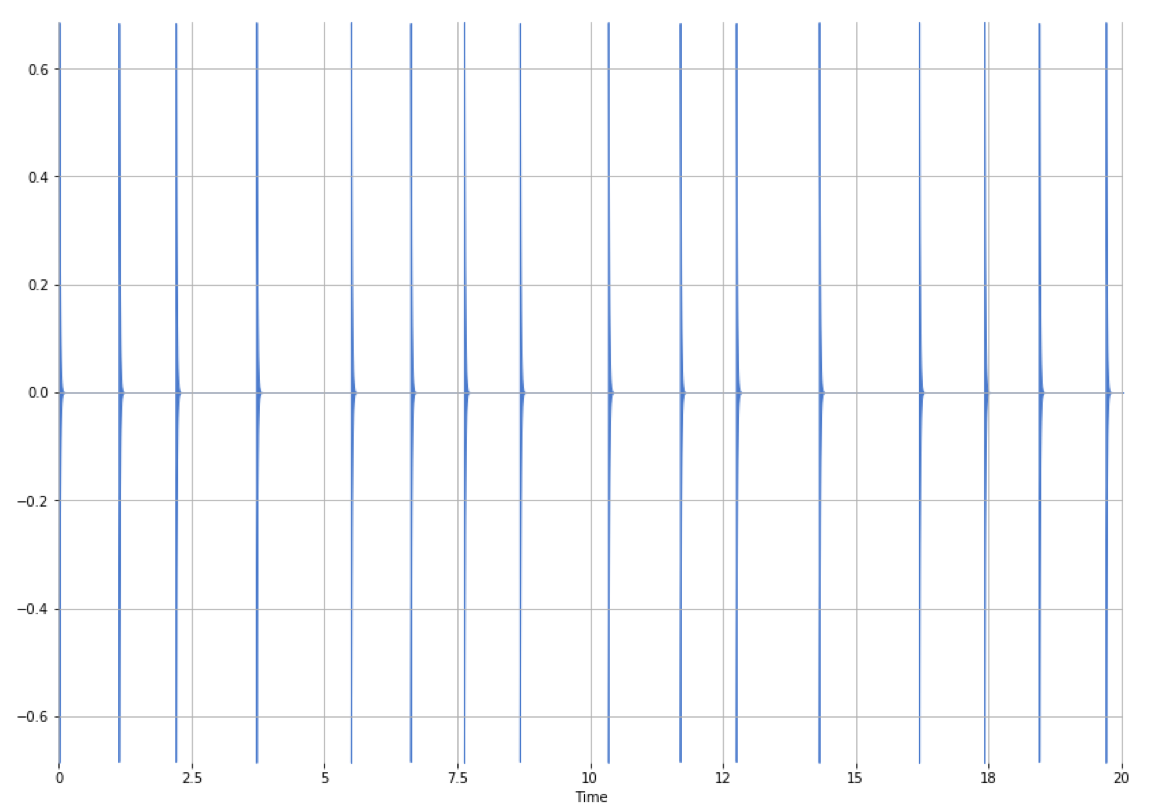
\includegraphics[width=0.5\columnwidth]{Click_waveform}}
        \subfloat[A3b1: interstitial tone]{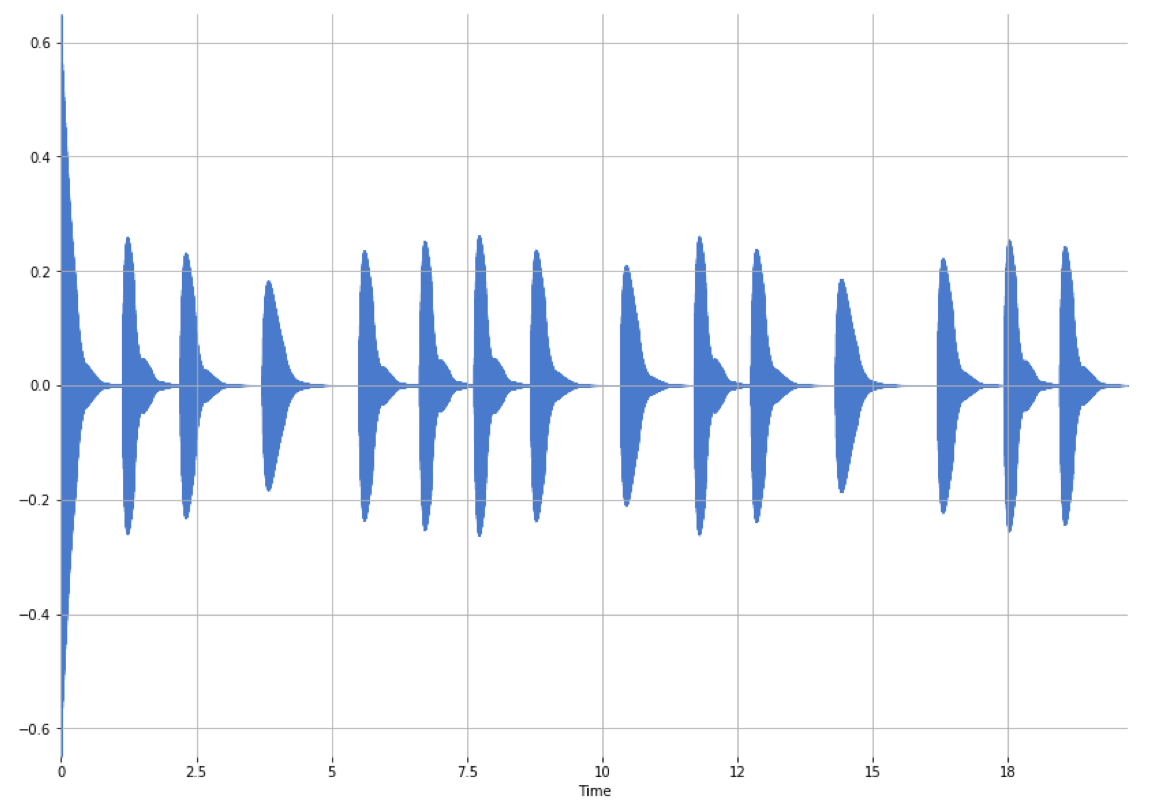
\includegraphics[width=0.5\columnwidth]{SwingClick_waveform}}
    \label{fig:click_comparison}
\end{figure}

\subsubsection{Stacatto and legato melody}
As a specific musical listening task, test cases \textbf{A2a}, \textbf{A4a} and \textbf{A2b}, \textbf{A4b} involve synchronization to a simple melodic sequence of notes. The music chosen was the nursery rhyme \textit{Pat-A-Cake}. The initial mockup was drafted in Sibelius and exported to Logic Pro X for bpm adjustment.

Each quarter note represents a beat and therefore a 1:1 synchronization tap onset task. In order to emphasize a discrete event for test cases \textbf{A2a} and \textbf{A4a}, notes were input as stacatto, shown below in Figure \ref{fig:patacakea2a}.

\begin{figure}[H]
    \centering
    \includegraphics[width=\textwidth]{Pat-a-Cake_a2a}
    \label{fig:patacakea2a}
\end{figure}

The interstitial counterparts (\textbf{A2b}, \textbf{A4b}) similarly underwent crescendo and decrescendo after every note onset with forte accents surrounded by mezzopiano to give the impression of amplitude build up and decay, shown below: \ref{fig:pat-a-cake_a2b} 

\begin{figure}[H]
    \centering
    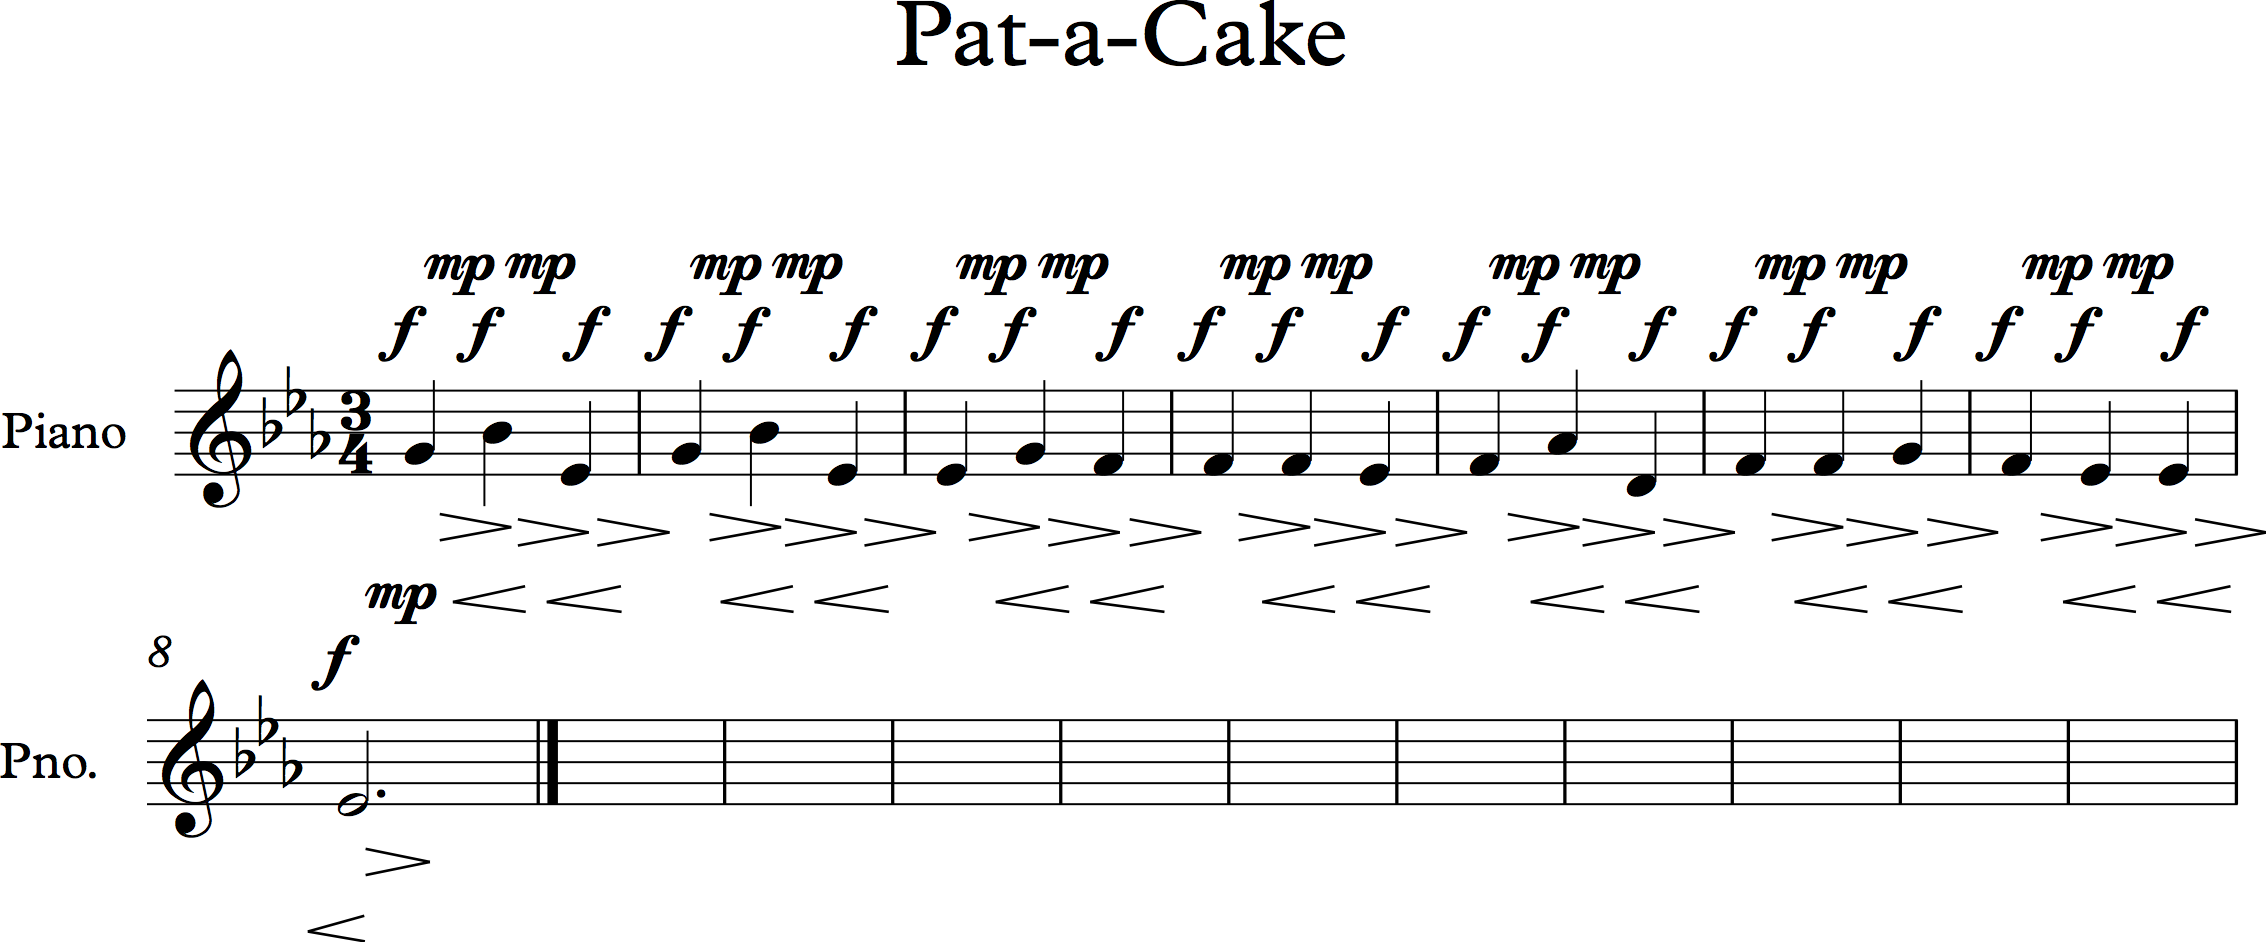
\includegraphics[width=\textwidth]{Pat-a-Cake_A2b}
    \label{fig:pat-a-cake_a2b}
\end{figure}

Note below in Figure \ref{fig:music_comparison} the gradual, nearly exponential decay displayed in the interstitial tone as a result of the legato input along with the amplitude difference due to the forte accents.

\begin{figure}[H]
    \centering
    \caption{Musical waveform comparison}
        \subfloat[A2a1: stacatto melody]{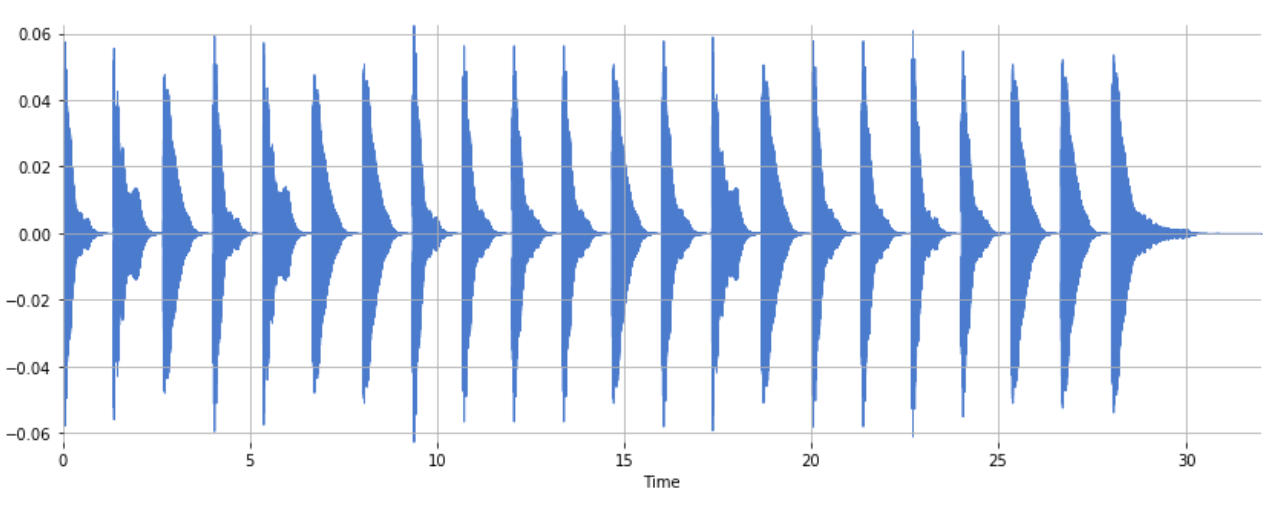
\includegraphics[width=\columnwidth]{A2a1_waveform}}
        \qquad
        \subfloat[A2b1: legato melody]{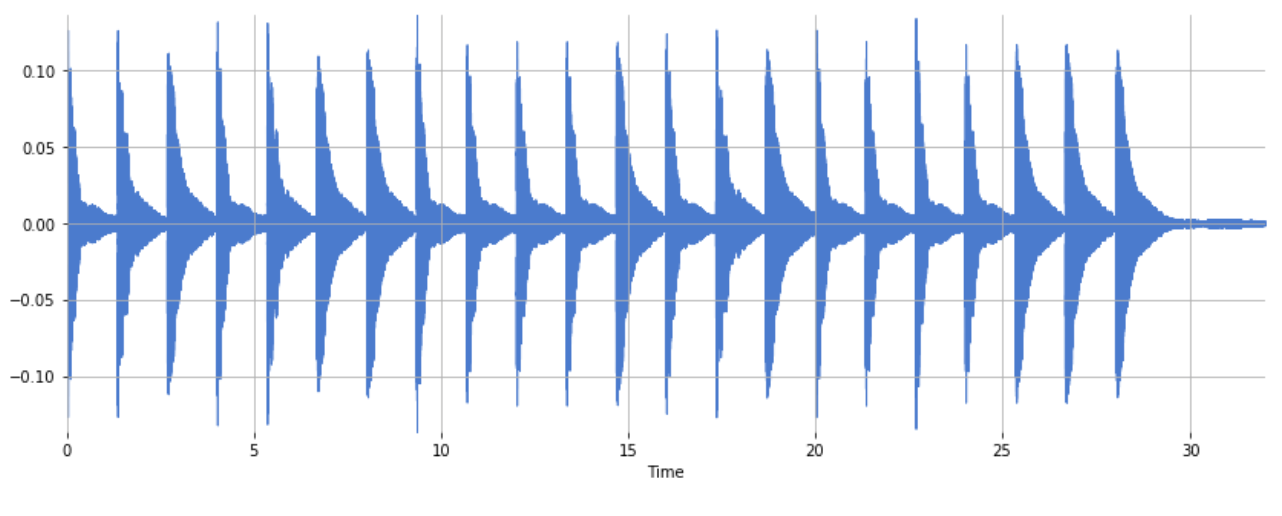
\includegraphics[width=\columnwidth]{A2b1_waveform}}
    \label{fig:music_comparison}
\end{figure}

\subsubsection{Dynamic tempi manipulation - audio}
Dynamic manipulation of tempo was accomplished in \textit{Logic Pro X} through automation of the tempo parameter over the time period of the desired waveform. Each test case started on one of the pre-defined BPM's (45, 90, 135, 180) but traversed either sinusoidally or triangularly through segmented time blocks as peaks and troughs ranging plus or minus 15 bpm; shown in \ref{fig:dynamic_audio}.

\begin{figure}[H]
    \centering
    \caption{Dynamic audio tempo automation patterns}
        \subfloat[45 +/- 15]{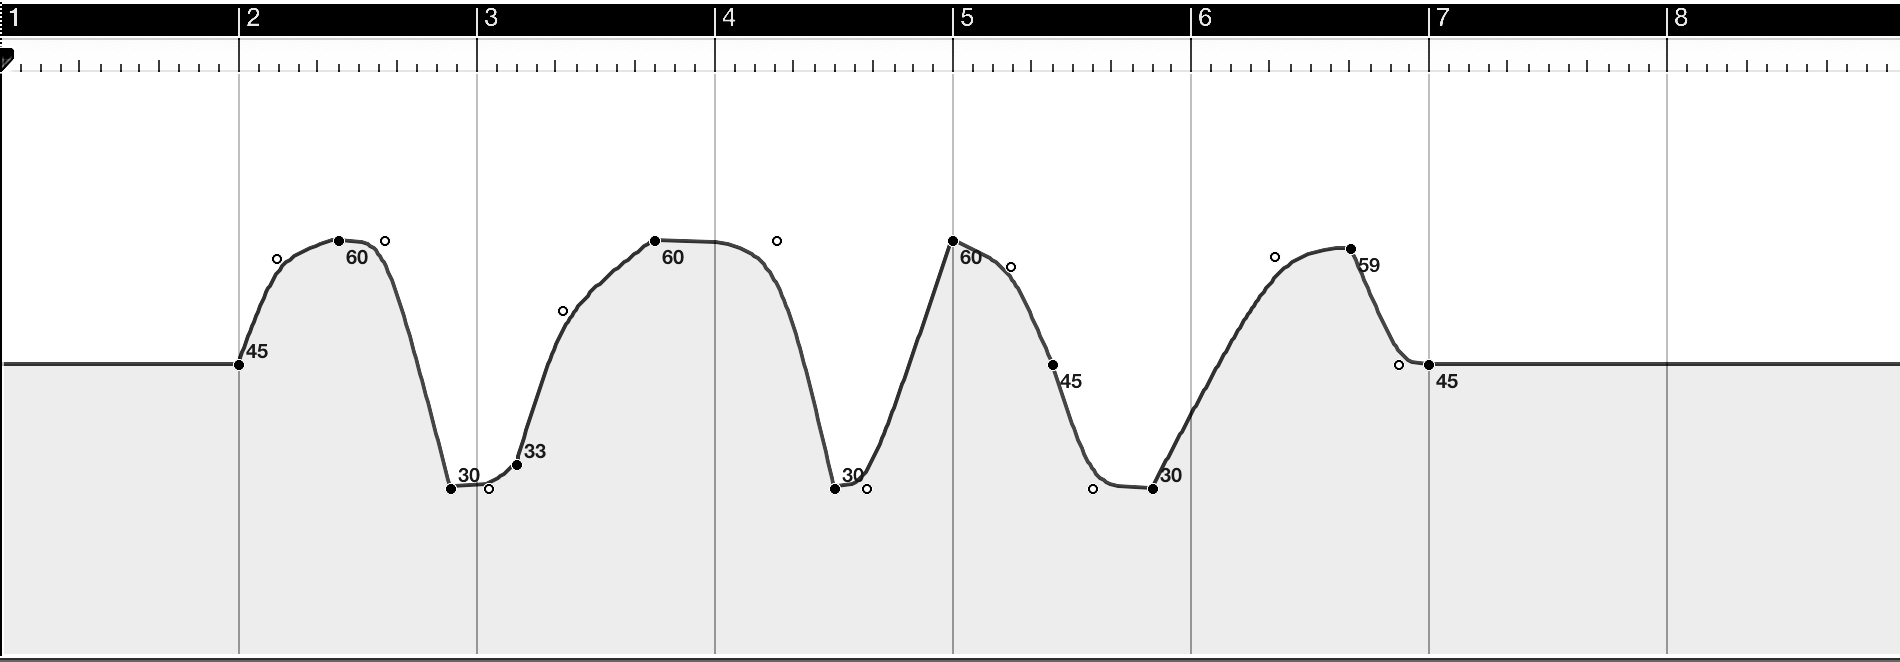
\includegraphics[width=.5\columnwidth]{dynamic_45}}
        \subfloat[90 +/- 15]{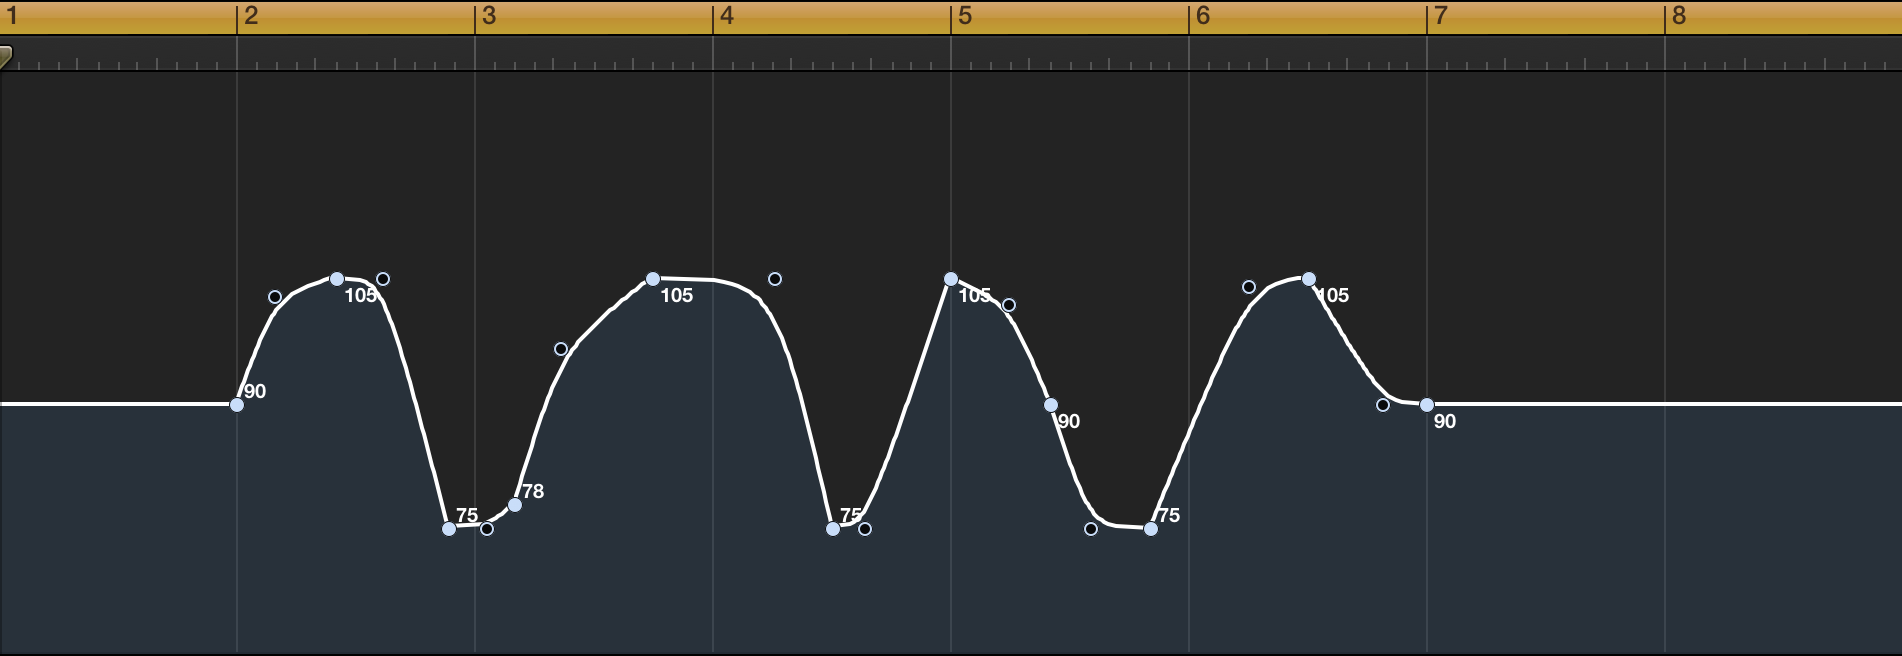
\includegraphics[width=.5\columnwidth]{dynamic_90}}
        \qquad
        \subfloat[135 +/- 15]{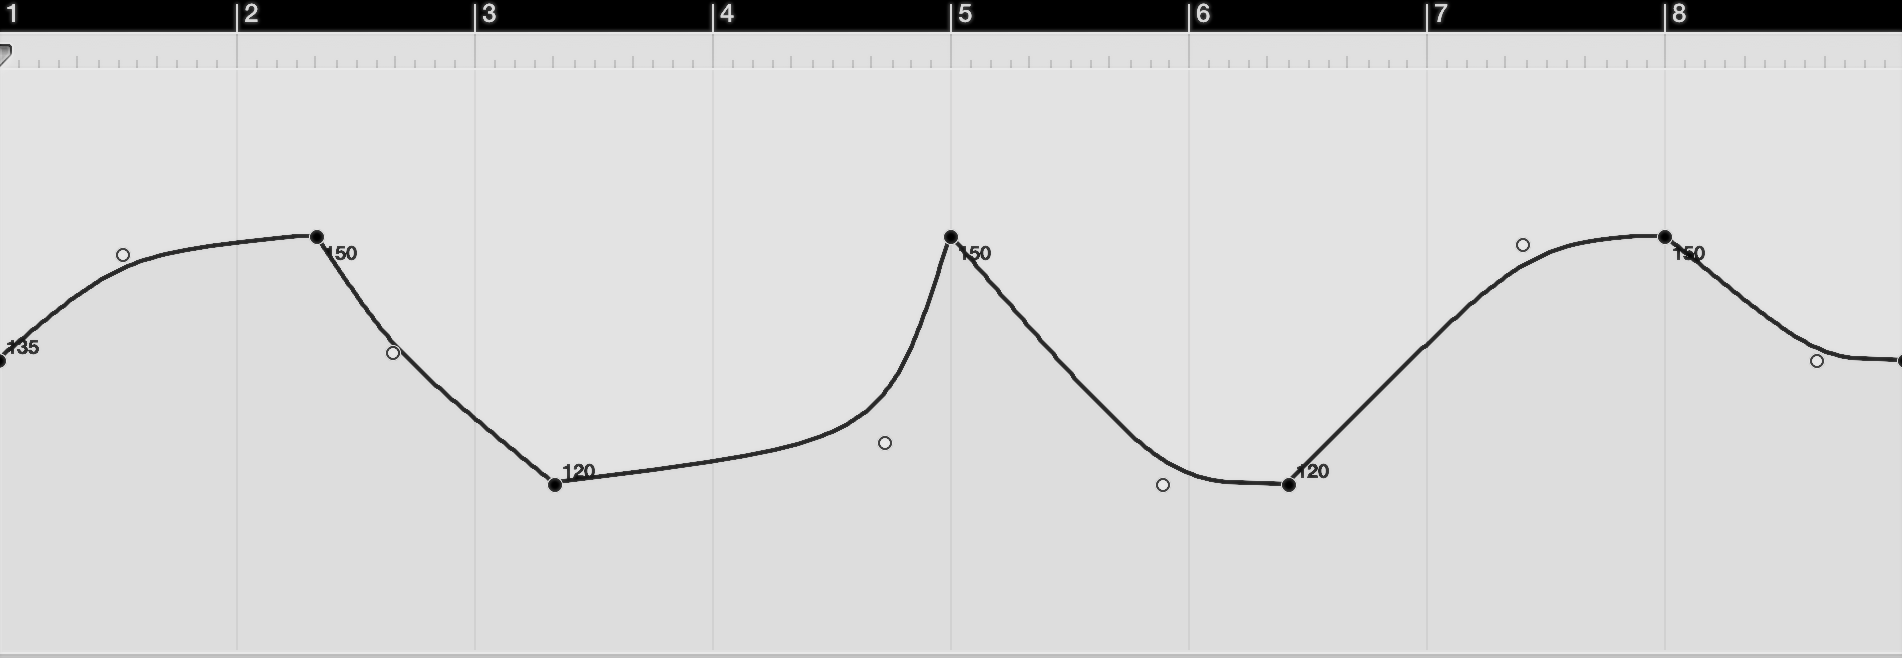
\includegraphics[width=.5\columnwidth]{dynamic_135}}
        \subfloat[180 +/- 15]{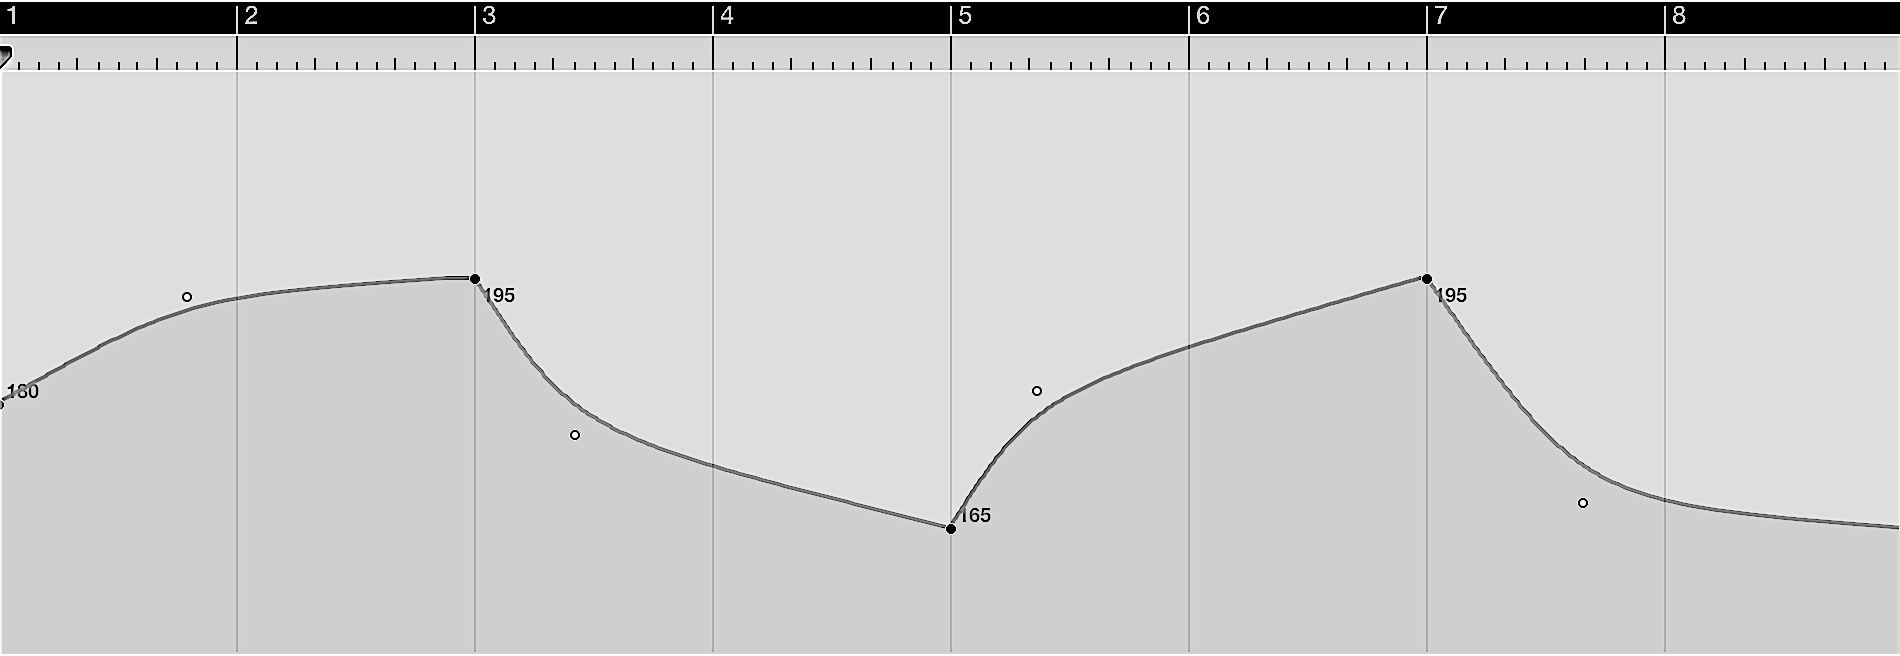
\includegraphics[width=.5\columnwidth]{dynamic_180}}
    \label{fig:dynamic_audio}
\end{figure}

\section{Test Suite}
High precision data acquisition and the minimization of delay were the central foci of the test suite design. Due to the extensive amount of publicly available libraries, multithreading capability, pandas dataframe structure, and plot integration via matplotlib, \textit{Python} was chosen as the development environment. Complementary to the software platform was the implementation of a tap onset detection mechanism via force sensitive resistor (FSR) and the \textit{Arduino Uno}. 

\subsection{Software Development} \label{development}
A high level breakdown of the framework is provided below.
\todo[inline]{fill out section}
            Discuss code breakdown

            Talk about how the logging was done:
                Knitty gritty details on where timestamps were
                vs.
                Justification on why time sync effort was not necessary
            
            GUI
            
            Haptic onset detection
            
            Tap onset detection
            
            Multithreading
            
            Audio onset detection
            
            Plotting

\subsection{Tap Onset Hardware}    \label{tap_arduino}
\todo[inline]{fill out section}

\subsection{Setup} \label{testSetup}
To initialize setup, the subject is seated and given a pair of closed-back headphones. The FSR is situated to their preference, either dominant or non-dominant hand, and secured into place. Unlike a keyboard or button the FSR gives little to no feedback or rebound. This ensures a confident tap on each onset while providing no tactile response. The approach seeks to avoid intrinsic lag due to its independence of mechanical components. The delay limit is defined by the threshold applied in the software to avoid debounce, as discussed in Section \ref{development}

\begin{figure}[H]
    \centering
    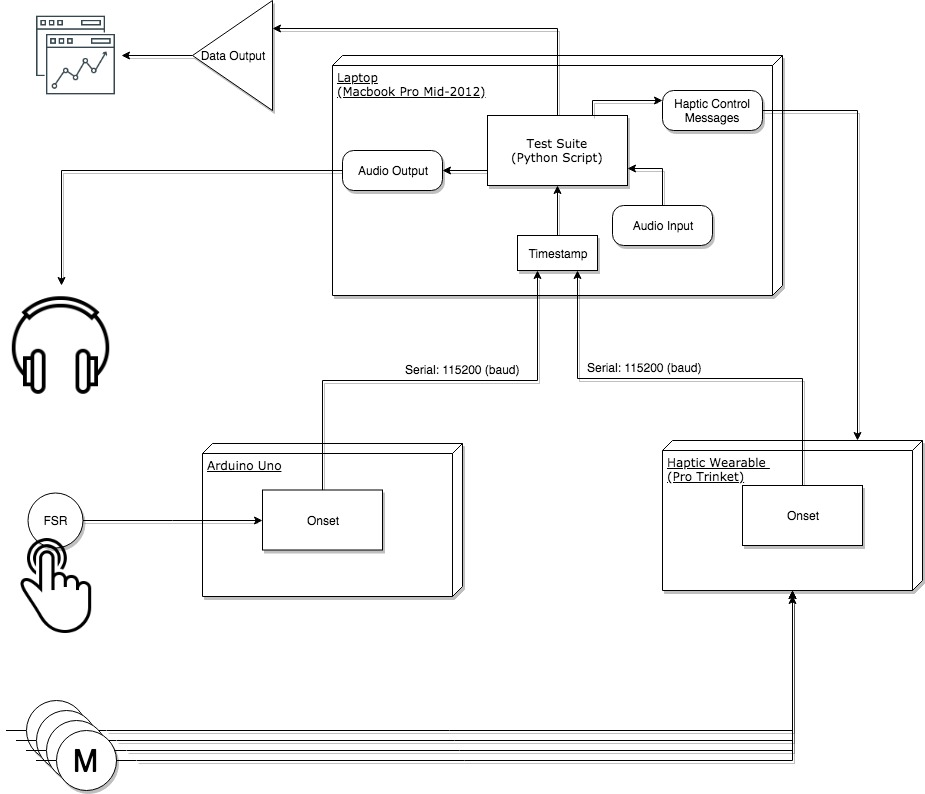
\includegraphics[width=\columnwidth]{TestSuiteFlowDiagram}
    \caption{Test Suite Flow Chart}
    \label{fig:TestSuiteFlowDiagram}
\end{figure}

The Python file \textit{testSuite.py} is run and the UI will prompt the subject to input their name, read the instructions, agree to the conditions of the test suite, and commence with the test. The first 8 are practice tests to get used to the haptic sensation as well as the variety of audible test cases. The order of test case execution is scrambled with a static seed pseudo-random generator such that every user encounters the same test order. Every iteration of the test plots the Tap Onset, True Onset, and Sanitized Onset  for the purposes of feedback and affirmation of correct tapping as seen in Figure \ref{fig:TestCaseFeedbackEx}. Upon completion of the 48 test cases, the users are asked to fill out a survey for feedback.

\begin{figure}[]
    \centering
    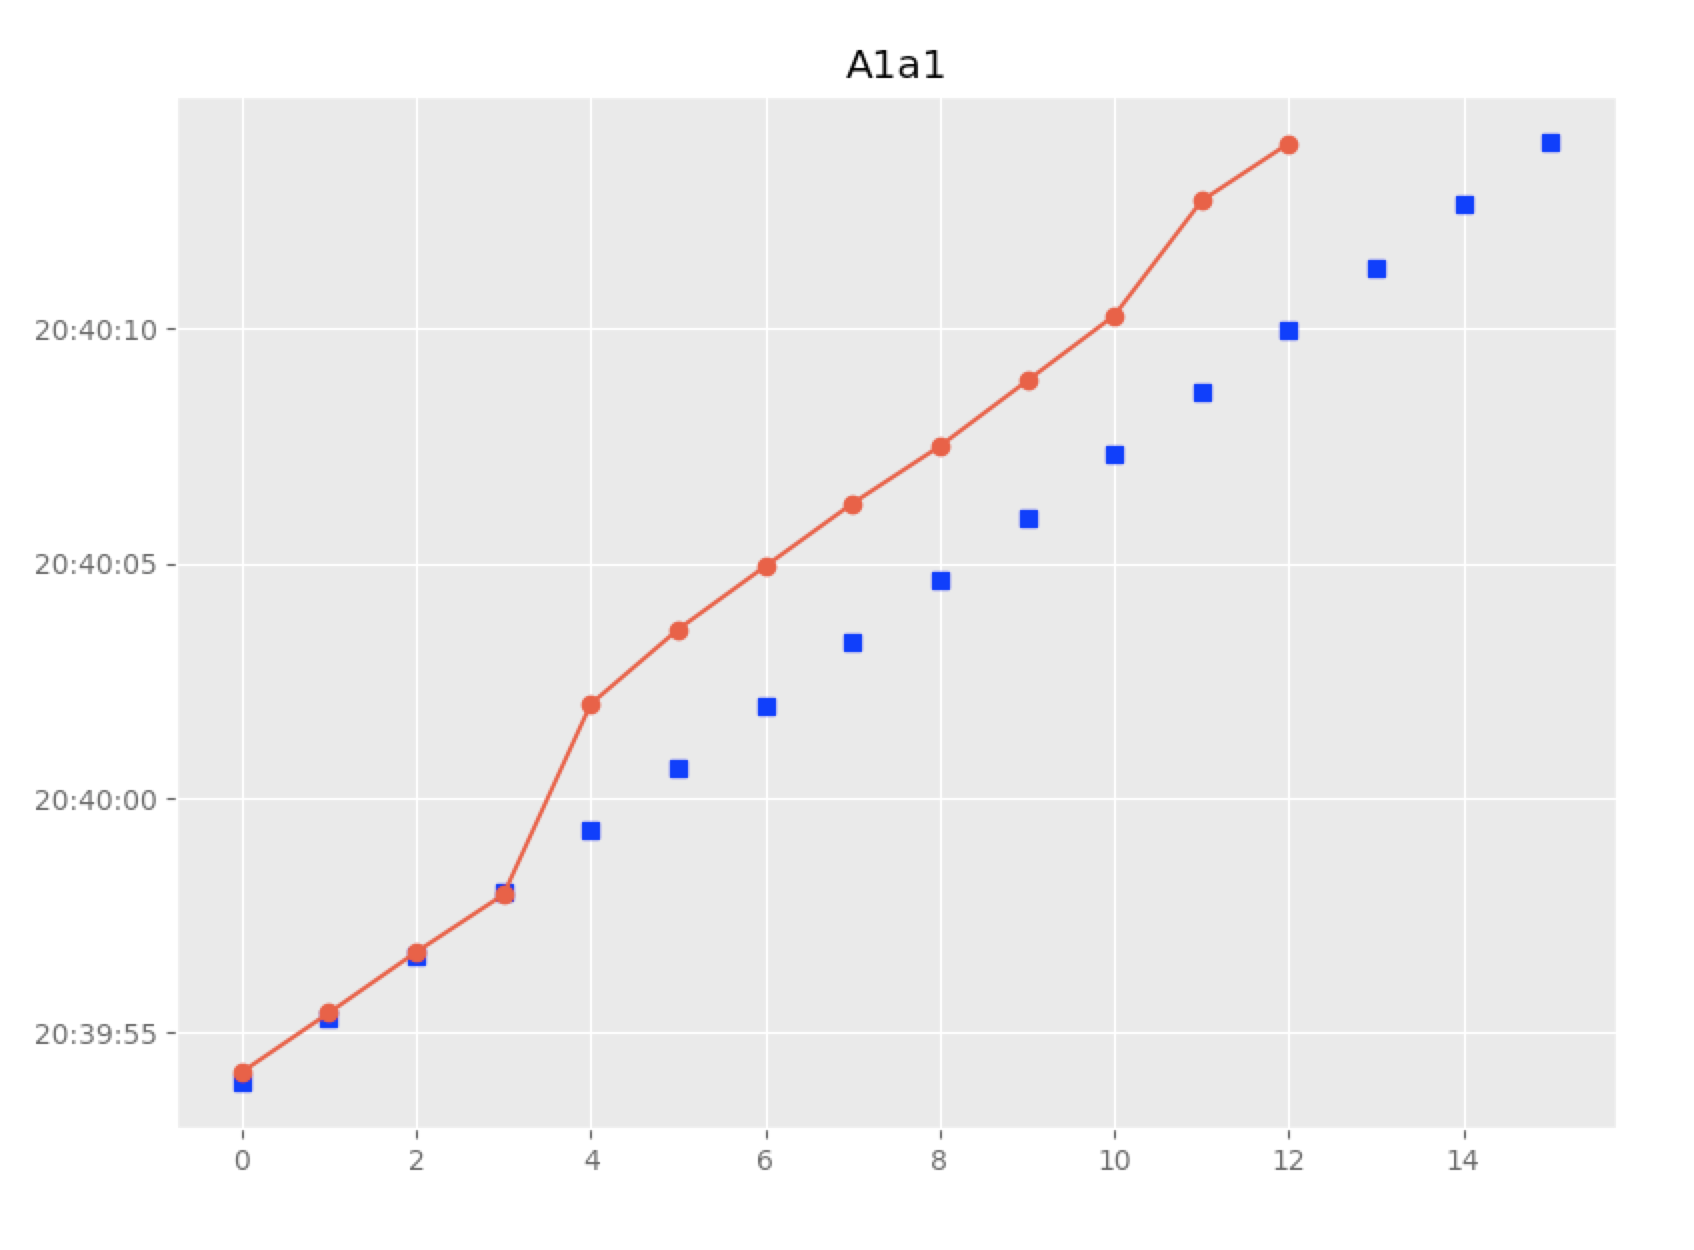
\includegraphics[width=\columnwidth]{TestCaseFeedbackExample}
    \caption{Test Case Feedback Example}
    \label{fig:TestCaseFeedbackEx}
\end{figure}

\subsection{Latency Evaluation} \label{latencyCalc}
Significant effort was placed in determining the overall latency of the test system to instill a level of confidence in the validity and accuracy of the data points acquired. The sources of potential latency were isolated into the components identified below.
\begin{itemize}
    \item FTDI-USB Communication
    \begin{itemize}
        \item According to section 3.1 of the datasheet for FTDI based chipsets\footnote{\url{http://www.ftdichip.com/Support/Documents/AppNotes/AN232B-04_DataLatencyFlow.pdf}} , FTDI USB-Serial communication to PC exhibits by default a round trip delay of 16 ms intrinsic to the packet scheduler. When the latency timer expires and the buffer is not yet full any data in the 62 byte buffer is sent along with a short 2 byte status message (total of 64 bytes).
    \end{itemize}
    \item USB $->$ Arduino Uno $->$ Laptop
    \item 50 ms vibrotactile motor ramp up time (see Appendix)
    \item Pro Trinket Haptic Onset Trigger Message (True Onset) $->$ PC $<-$ Tap Onset
    \begin{itemize}
        \item In order to quantify latency within the haptic design tests were repeatedly run within a closed loop environment. This meant that the onset trigger I/O pin at the gate node of the Pro Trinket was connected to the A0 pin on the Arduino Uno, emulating the same effect as a tap of the FSR.
        \item Force Sensitive Resistor
            * analog read/mention debounce threshold
            * transmit time
                * human input is never perfect, above the noise floor but just enough to get the input
        \item Constant offset:  
            * Within the haptic codes dual states of operation there exists two sources of error within the state machine. 
                * The onset trigger in discrete mode starting $1/4$ of a period after 
        \begin{lstlisting}[language=C]
            if((millis()-startTime) >= ((average * 1)/4))
            {
                newState++;
                Serial.println("onset");
            }
        \end{lstlisting}
    \end{itemize}
    \item Audio engine playback
    \item python thread time
        * intrinsic jitter when that many asynchronous processes together
        * File I/O
\end{itemize}
The overall summation was applied to each data point in the final analysis.

